\chapter{Introduction}\label{ch:intro}

\quote[0.625\textwidth]{Eventually everything connects - people, ideas, objects. The quality of the connections is the key to quality per se.}{Charles Eames}

How much do the votes of politicians reflect their party affiliations? Stokes writes that ``political parties are endemic to democracy''~\cite[p.245]{stokes1999}, so wondering about the empirical expression of party beliefs is important to diagnose issues in the democratic process. It helps inform the debate of whether political parties ``made modern democracy'', contributing to its responsiveness and realization of public good, or ``are an inextricable weed'' in democracy's garden, ``partial to their own conception of the good''~\cite[pp.263--264]{stokes1999}. In Switzerland, the National Council is one of the main stages of federal politics~\footnote{It is one of the two houses that form the Federal Assembly of Switzerland, the other being the Council of States.}. Since 1963, it has had a fixed number of seats (200) divided into shares proportional to each canton's percentage of the total population. Every four years the Swiss people elects a new council, the most recent of which has held office from 2015 to 2019. It is the 50th legislature since the foundation of the Swiss federation, in 1848. Figure \ref{fig:snc_photo_and_parties} displays a photo of the Council hall, next to a scatter plot of the National Councillors taking part in the 50th legislature, highlighting their party affiliations.
\begin{figure}[H]
    \centering
    \subfloat[The Council hall at the Federal Palace in Bern, Switzerland. \textcopyright \, 2006 \url{http://www.parlament.ch}]{
        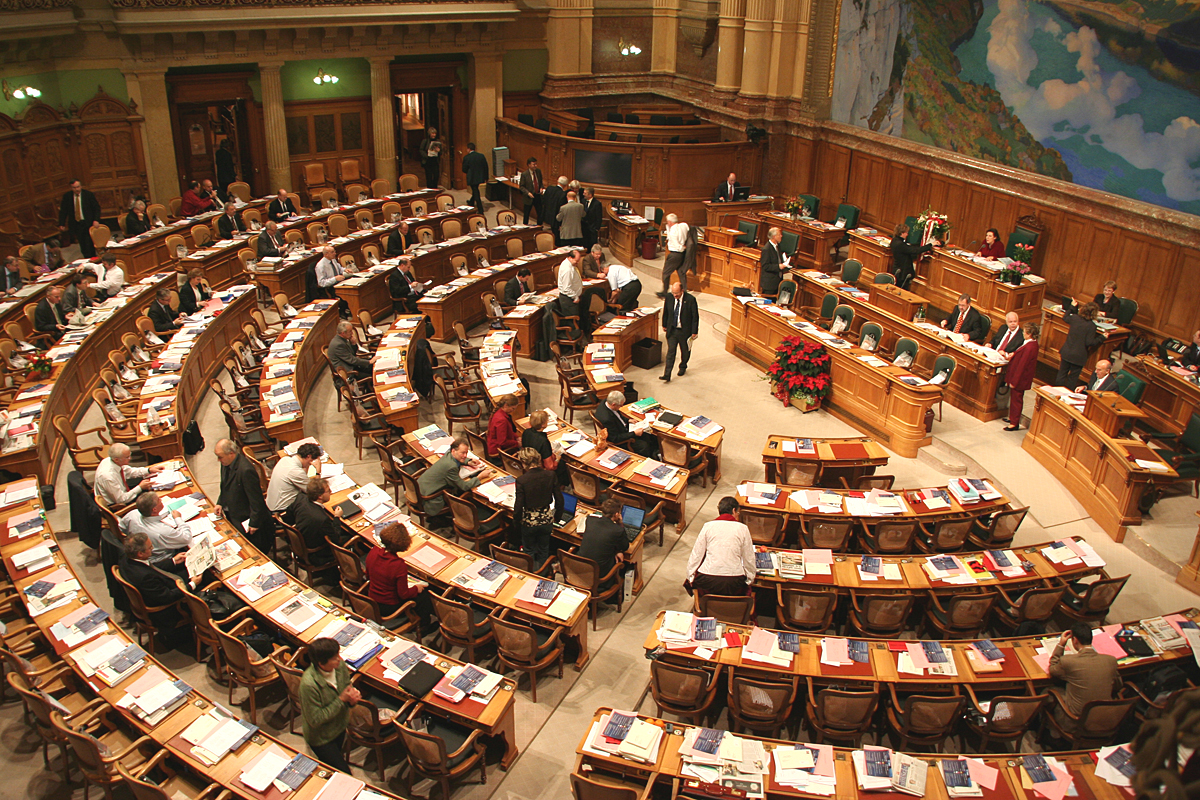
\includegraphics[width=0.5\textwidth]{snc_photo.jpg}
        \label{fig:snc_photo}
    }
    \hfill
    \subfloat[Council members and their party affiliations during the 50th legislature.]{
        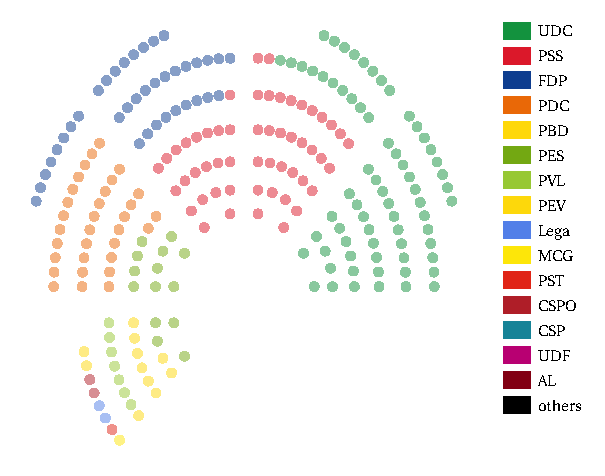
\includegraphics[width=0.45\textwidth]{snc_parties_no_edges.pdf}
        \label{fig:snc_parties_no_edges}
    }
    \caption[The Swiss National Council]{The Swiss National Council. The scatter plot on the right has more ``chairs'' than the 200 in the actual council hall on the left because I account for councillors that resigned or were replaced throughout the 50th legislature.}
    \label{fig:snc_photo_and_parties}
\end{figure}

The Swiss Parliament has an Open Data policy, allowing --- in particular --- the consultation of voting results through a database of parliamentary votes~\footnote{See \url{https://www.parlament.ch/en/ratsbetrieb/abstimmungen/abstimmungs-datenbank-nr}. I was pointed to this source by  D. Debruyn, Y. Morize, N. Orgland, and S. Stettler, who were all EPFL Master's students at the time.}. With this data, we can find out how each National Councillor voted in each of the affairs in the 50th legislature, and, comparing the voting patterns, record how similar the councillors are to one another in their voting behaviors. I depict these similarities in the form of a network (or graph) on Figure \ref{fig:snc_parties_with_edges}, with edges connecting councillors who voted the most alike during the period 2015--2019.~\footnote{I disclose the precise way in which this graph is constructed only in Chapter \ref{ch:numerical_tour}. For now, it suffices to interpret connected vertices as representing councillors with similar voting decisions.} Despite increasing polarization of the Council since the 1990s --- tied to the rise of the right-wing UDC party~\footnote{\url{https://www.swissinfo.ch/eng/political-drift_polarisation-of-swiss-parliament-continues/43752300}} --- it is not rare to find in Figure \ref{fig:snc_parties_with_edges} councillors from different parties that nonetheless vote alike. Had the Council been completely polarized, vertices of different colors would never connect. Still, party affiliation is not meaningless, as there seems to be more connections within than across parties. But how much of the party division in the Swiss National Council is encoded in the network structure induced by the voting data? Or, more concretely, if we knew the party affiliations of half the councillors, as in Figure \ref{fig:snc_subsampled_parties_with_edges}, could we infer the other half of the labels based on the connectivity information?

\begin{figure}[H]
    \centering
    \hfill
    \subfloat[The graph with all the party labels.]{
        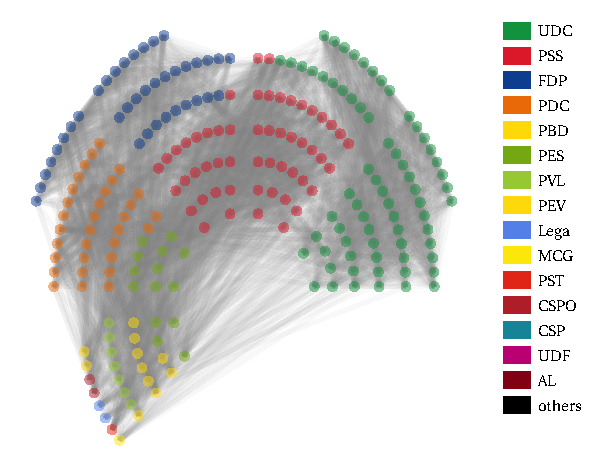
\includegraphics[width=0.45\textwidth]{snc_parties_with_edges.pdf}
        \label{fig:snc_parties_with_edges}
    }
    \hfill
    \subfloat[The graph with half the party labels.]{
        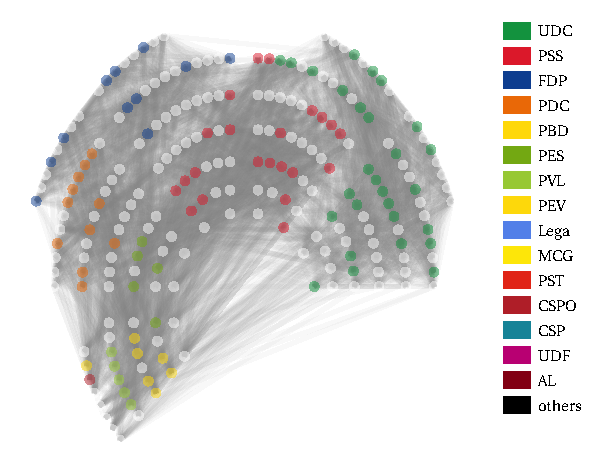
\includegraphics[width=0.45\textwidth]{snc_subsampled_parties_with_edges.pdf}
        \label{fig:snc_subsampled_parties_with_edges}
    }
    \hfill
    \caption[The voting-similarity graph for the Swiss National Council]{The voting-similarity graph for the Swiss National Council. Each vertex represents a council member, and the edges connect members that had similar voting patterns during the 50th legislature.}
\end{figure}

These musings are part of the usual pipeline in modern Data Science~\cite{vanderaalst2016}. An object of interest in the real-world (Swiss National Council) has some available data (vote results) that can be used to infer some property (party labels) of the object in question. The need for such inference may come from difficulties in measuring the desired property or simply out of scientific interest on the predictive powers of the available data. In the contrived example of the missing party labels in Figure \ref{fig:snc_subsampled_parties_with_edges}, we might be just interested to see if the voting patterns reflect the party affiliations. But in graphs such as the Internet or large social networks querying every single node for some property can be very expensive. The missing information in these cases is intrinsically due to the large size of the network. To infer, or recover, the full content from scarce observations, there are two main issues that practitioners concern themselves with. First, which kind of --- and how many --- measurements are available. Second, which machinery to use to retrieve the missing information. The first point pertains to what I call the \emph{sampling} stage of the pipeline; the second, to the \emph{decoding} stage. In this thesis, I assume the freedom to act in both, choosing a suitable decoder for an important class of signals, and subsequently looking for an optimal sampling strategy adapted to this decoder. Optimality here refers to reducing the number of measurements needed from the sampling stage for a successful decoding stage. An added benefit of studying optimal sampling lies in the possibility to quantify how suited the decoder is in retrieving the signals of interest. The more samples the decoder needs, the less suited it is. Take, for example, the Swiss National Council data, and imagine we chose a decoder for missing party labels (like those of Figure \ref{fig:snc_subsampled_parties_with_edges}) based on the voting-similarity connections. This decoder's optimal number of samples could therefore function as a numerical proxy to how well the councillors' votes echo their party affiliations.


\section{The main objects and questions in the thesis}

Networks (or graphs) have long been objects of interest in Mathematics and Computer Science, but they have found their way into Signal Processing over the last decade or so. \acrfull{gsp} is now an established subfield~\cite{shuman2013, sandryhaila2013a, ortega2018}, concerned with any quantities whose support can be interpreted as being a graph. As a matter of fact, I have already shown a graph signal. Each member (vertex) of the Swiss National Council  was associated with a party color, so we can understand the mapping ``councillor $\mapsto$ color'' in Figure \ref{fig:snc_subsampled_parties_with_edges} as a signal living on the voting-similarity graph. On the Internet, a relevant signal is the number of data packets at each router; on a social network, it might be people's likelihoods of buying a given product. Even when a graph is not naturally present --- as in the Swiss National Council example ---, representing the variable dependencies through a network may be a beneficial pre-processing step. To connect a vertex to only a few neighbors is akin to statistical selection, restricting a variable's predictors to its most similar peers. Moreover, these few connections implicitly constrain the interactions between vertices to happen only locally, so comparisons of signal values can be more efficiently computed.

One of the central tenets of \acrshort{gsp} can be stated as ``connected vertices have similar signal values''.~\footnote{An analogous statement, ``similar variables have similar outputs'', is the central assumption of the related field of Semi-Supervised Learning~\cite{chapelle2006}.} It is the glue that binds the graph and the signals that it supports, but it gives room to specify what ``similar values" means. This thesis deals with a particular set of graph signals deemed \emph{piecewise-constant}. In loose terms, these objects assume constant values over sizeable swathes of the graph, but are allowed to vary abruptly between the constant pieces. The councillors colors in Figure \ref{fig:snc_subsampled_parties_with_edges} is an example of piecewise-constant signal: each party defines a piece of constant color, but those colors are allowed to vary abruptly between pieces. In general, any classification or segmentation task can be interpreted as producing a piecewise-constant signal on some graph. Indeed, imagine a social network, then assign value $1$ to every person who has watched the 2010 movie ``The Social Network'', and value $0$ otherwise. The $\{0,1\}$-valued labels thus defined form a piecewise-constant signal over the social network. Whenever we know the value of a signal at a vertex of the graph, I will say that this vertex has been sampled. Sampled vertices represent the knowledge that an oracle made available to us to help us figure out the full underlying signal. This thesis admits oracles that provide \emph{vertex samples independently at random}, according to a probability distribution set beforehand. They are a model for any stakeholder that has a budget number of samples with which to query the network for a signal of interest. Some vertices may be more important than others, so they could be sampled with higher likelihood; the samples are kept independent to facilitate the mathematical treatment of the process. Intuitively, if a company wants to sell a product, then ``influencers'' in a social network should definitely be queried for their propensity to advertise the merchandise. Readers will find in Chapter \ref{ch:graphs_signals_sampling} all the formalism that I use in subsequent chapters when speaking of graphs, signals on graphs, and the sampling of these signals.

\begin{wrapfigure}{o}{0.35\textwidth}
    \centering
    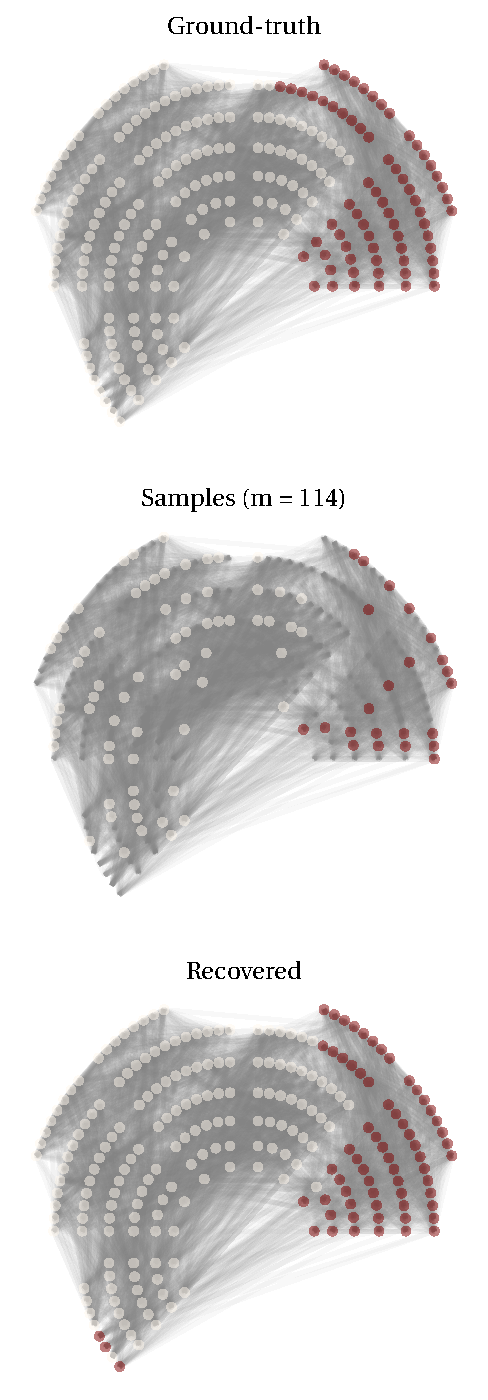
\includegraphics[width=0.3365\textwidth]{snc_sample_rec_example.pdf}
    \caption[The processing pipeline highlighting the sampling and decoding stages]{Example of the processing pipeline highlighting the sampling and decoding (recovery) stages. See the paragraph on the left for details.}
    \label{fig:snc_sample_rec_example}
\end{wrapfigure}

The decoders in this thesis manifest themselves in terms of \emph{convex programs}. That is, their output is chosen by minimizing some convex loss function. Piecewise-constant signals vary only across few of the edges on their graph support, so it makes sense to pair them with a recovery function that penalizes edge-differences.~\footnote{In a way, this recovery procedure is an instance of transductive learning \cite[Chapter 24]{chapelle2006} where the sampled vertices form the training set, the unsampled vertices the testing set, and the loss implicitly defines a search space.} This idea leads to the central subjects of the thesis, \acrfull{gtv} decoders. They are programs that minimize a semi-norm of the form $\|\mathbf{D} \cdot\|_1$, for some difference operator $\mathbf{D}$. \acrfull{tv} minimization is a standard tool for processing ``classic'' time-series or images that have rare, but sudden changes in value. Think here of a quantized waveform, or a Mondrian painting. I will show how \acrshort{tv} and piecewise-constant graph signals are also intimately related. Chapter \ref{ch:recovery_convex} provides the required background on convex recovery and introduces the \acrshort{gtv} decoders so central to this thesis.

The performance of the decoder depends on what happens at the sampling stage. To get a better feeling for this, let us revisit the Swiss National Council example, this time with a different graph signal. The top row of Figure \ref{fig:snc_sample_rec_example} depicts the indicator function of the Swiss People's Party (UDC in French), the largest party in the 50th legislature, occupying about 30\% of the total seats. The signal takes value $1$ (yellow) at vertices representing UDC members, and $0$ (blue) everywhere else. UDC is politically the farthest to the right on the National Council, so the party should be fairly well encoded in the voting patterns represented by the edges of the graph. In the middle row of Figure \ref{fig:snc_sample_rec_example}, I have sampled the UDC indicator function at 50\% of the vertices, uniformly at random. Many instances of both yellow (UDC) and blue (non-UDC) vertices appear in the sample because the party constitutes a considerable share of the Council. The third row of Figure \ref{fig:snc_sample_rec_example} shows the decoded signal as output by \acrshort{gtv} interpolation, yet to be introduced in Chapter \ref{ch:recovery_convex}. Most of the vertex labels are recovered correctly, but there are visibly wrong assignments. This means that sampling uniformly at random the labels of \emph{half} the councillors is still not enough to guarantee a perfect recovery using our decoder. Sampling uniformly at random, however, is not the only way to query the vertices under our oracle model. We could sample more often the vertices that are poorly connected, or sample more often the hubs of the graph, or even mix those two strategies. The possibilities are endless. Rather than think of an ad hoc plan of action, this thesis asks

\begin{center}
    \framebox[1.1\width][c]{%
        \parbox[t][44pt][c]{0.8\textwidth}{
            \centering
            What is the vertex sampling design that minimizes the number of measurements required for the success of \acrshort{gtv} decoders?
        }
}
\end{center}

The best hope one has to find a sampling design that answers the question above is by studying the conditions for successful recovery under \acrshort{gtv} minimization. In the course of this study, we will encounter typical concepts that usually arise when dealing with stochastic objects in high dimensions~\cite[Ch. 1]{vanhandel2014}, such as concentration, universality, and sharp transitions. In particular, I will show that the recovery error drops suddenly to zero (with a high likelihood) at a critical number of measurements that depends on the vertex sampling probabilities. Minimize this threshold and one can find the optimal sampling design.

\section{Contributions}

To prove that a convex program returns the desired output, one must produce a \emph{certificate}, an object whose very existence guarantees the success of the recovery procedure. Chapters \ref{ch:lower_bound_min_gain} and \ref{ch:inexact_dual} describe two parallel attempts that I made towards producing such guarantees.

In Chapter \ref{ch:lower_bound_min_gain}, the certificate manifests itself as a positive lower bound on a minimum gain functional. This view has proven fruitful when Gaussian-like vectors are used to measure the ground-truth signal, and has become standard in the literature~\cite{chandrasekaran2012, tropp2015a}. However the nature of vertex sampling gets in the way of the usual small-ball method~\cite{mendelson2015, koltchinskii2015} used to lower bound the minimum gain. As a result, I ultimately fail in this attempt, but I end the chapter pointing towards a possible redemption, reliant on better knowledge of the coordinate structure of a certain ``descent cone''.

The real win comes in Chapter \ref{ch:inexact_dual}, while seeking a \emph{dual} certificate for the \acrshort{gtv} decoder. There, the \acrlong{kkt} conditions of the problem motivate a blueprint for an iterative golfing scheme~\cite{gross2011} that produces, in the end, the desired recovery guarantee. It is this chapter that the number of measurements implying a successful recovery is upper bounded by an expression that depends on the vertex sampling probabilities. The optimal sampling design then comes directly as a corollary. Interestingly, the sampling probabilities in this design depend on how each vertex perturbs the graph difference operator, restricted to the edges across which the piecewise-constant, signal-to-be-recovered changes in value.

Chapter \ref{ch:numerical_tour} closes the thesis with a numerical tour to balance out the mostly theoretical discussion up to that point. There I plot --- for a variety of graphs and signals of interest ---, the phase transition undergone by the recovery error of a \acrshort{gtv} decoder when the number of sampled vertices changes. Experiments show how these phase transitions can be improved using proper sampling designs, but the question of how to make proper designs that  are also \emph{practical} remains open by the end of the book.

\section{The presentation of the proofs}

Most chapters in this thesis contain theorems with somewhat lengthy proofs, whose immediate presentation would disturb the flow of the text. For this reason, I have gathered detailed arguments largely in appendices at the end of the relevant chapters. The proofs themselves are written in a hierarchical structure, based on the guidelines of L. Lamport~\cite{lamport2012}. For the unfamiliar reader, this means that I build a sequence of discrete, provable claims leading to the desired result. Each of these discrete claims are settled as true either by appealing to established knowledge, or by presenting a sequence of discrete sub-claims. In the end, the full proof resembles a nested list. I have avoided too much nesting due to the obvious limitations of the printed format. Still, the hierarchical structure should make it easier to distill the arguments and find exactly where I use each assumption in the statement of their respective theorems.

\section{Reproducibility and Open Science}

\begin{minipage}{\textwidth}
    {%
    \setlength\intextsep{0pt}
        \begin{wrapfigure}{i}{0.15\textwidth}
            
\includegraphics[width=0.16\textwidth]{cc-by.png}
        \end{wrapfigure}
    %
    \noindent This work is licensed under a \href{http://creativecommons.org/licenses/by/4.0/}{Creative Commons Attribution 4.0 International License}. All the computer code required to reproduce the contents of this thesis is distributed under the \href{https://opensource.org/licenses/MIT}{MIT License}, and hosted at the following repository:
    %
    \begin{center}
        \framebox[1.1\width][c]{%
            \parbox[t][22pt][c]{0.5\textwidth}{\url{https://github.com/rodrigo-pena/phd-thesis}}
    }
    \end{center}%
    }
\end{minipage}
